%\documentclass[a4paper,11pt]{article}
%\usepackage[T1]{fontenc}
%\usepackage[utf8]{inputenc}
%\usepackage{lmodern}
%\usepackage{graphicx}
%\begin{document}

\section{Research into Human Behaviour}
\label{Res:sec:humanBehaviour}
\subsection{Non-adaptive Behaviour}
\label{Res:subsec:nonadaptive}
Adaptive behaviour is any behaviour is any behaviour ``which contributes directly or indirectly to an individuals survival''.
Conversely non-adaptive behaviour is any behaviour which may be counter productive to an individuals survival \cite{AdaptiveBehaviourWiki}.
In the context of an evacuation this refers to high risk actions which occur in a crowd such as stampede, pushing and shoving others,
trampling others, etc.\\
The introduction of non-adaptive behaviour can be connected to the stress a person is feeling. More specifically, Law et al \cite{CIFEResearchProposal} propose that there are three factors which contribute to the emergence of adaptive or non-adaptive behaviour:
\begin{itemize}
  \item{\textbf{Panic}: when a person perceives danger they are more likely to make irrational decisions based on instinct \cite{PanMASSEgressThesis}.}
  \item{\textbf{Decision-making}: although panicked, a person is still capable of making rational decisions. This increases the likelihood of the individual making adaptive choices, such as correctly recognising an exit or refraining from shoving upon exiting.}
  \item{\textbf{Levels of urgency to exit}: individuals within a group will experience varying levels of arguing to leave the environment based on the level of danger they perceive themselves to be in. High urgency causes individuals to behave aggresively and prioritise self-preservation.}
\end{itemize}
All of these theories provide insights into human behaviour but have yet to be unified into a comprehensive theory.

\subsection{Bounded Rationality}
\label{Res:subsec:nonadaptive}
Bounded Rationality can be expressed as the principle that in a given situation the rational decisions a person can make are bounded by the set of possible options available to them and the time in which they can make a decision. This concept was initially proposed by Herbert Simon, who highlighted two interlocking components of bounded rationality \cite{BoundedRationalityDefinition}:
\begin{itemize}
  \item{\textbf{The limitations of the human mind}: the human mind does not have limitless processing power or memory and so must use approximate methods to handle most tasks. For computational purposes these methods can be expressed using simple heuristics.}
  \item{\textbf{Environmental structure}: Simon emphasised that the heuristics used must be adapted to the environment in which the decision is made.}
\end{itemize}
An important example of this priciple is Simon's concept of satisficing: a ``method for making a choice from a set of alternatives encountered sequentially when one does not know much about the possibilities ahead of time'' \cite{BoundedRationalityDefinition}. In an evacuation a person will use this satisficing technique to make decisions such as where to move next based on what they can see.\\
It is important to note that, like other rational behaviours, this process can be disrupted by the introduction of stress factors, as previously discussed.

\subsection{Conformity \& Social Proof Theory}
\label{Res:subsec:socialProof}
Conformity can be defined as a "change in behaviour or belief toward a group as a result of real or imagined group pressure". This can be further divided into \emph{normative influence} and \emph{informational influence}. Normative influence refers to changes in behaviour for the sake of winning the approval of other group members. Informational influence refers to conforming in an attempt to improve one's knowledge of reality and current situation. \cite{HandbookOfPsychology5}.\\
Informational influence, which is often called Social Proof Theory \cite{SocialProofWiki},  has the effect that when facing a situation with uncertainty, a person may turn to the surrounding group for cues. Cialdini noted ``we seem to assume that if a lot of people are doing the same thing, they must know something we don't'' \cite{PanMASSEgressThesis}.\\
This principle is at the core of many of the behaviours observed in evacuations, particularly herding behaviour \cite{PanMASSEgressThesis,MultiAgentFramework}.

\subsection{Personal Space}
\label{Res:subsec:personalSpace}
According to Edward T. Hall \cite{HiddenDimension} the space surrounding a person can be divided into four ``reaction bubbles'' which represent an acceptable radius around the person in which different categories of interaction. These are:
\begin{itemize}
  \item{\textbf{Public Space}: this space is used for speeches or other interactions with large audiences. This includes anything beyond roughly 2.4m}
  \item{\textbf{Social Space}: the distance reserved for interaction with strangers or newly formed groups. This ranges from around 1.2m to 2.4m}
  \item{\textbf{Personal Space}: this begins an arms length away from the individual's center and is reserved for interactions with friends or other close associates}
  \item{\textbf{Intimate Space}: The smallest of the spaces, this ranges from touching the person to around 50cm from their body. Interactions in this space are extremely personal and normally occur only with close members of family or friends}
\end{itemize}
The last two of these spaces are of particular interest. Another definition of personal space is the area surrounding an individual ``into which others may not intrude without causing discomfort'' \cite[pg. 424]{HandbookOfPsychology5}.\\
In a crowded environment the violation of ones personal space is likely to increase stress and anxiety (see page \pageref{subsec:personalSpace}. Naturally this effect is even greater when the intimate space is violated. An individuals desire to re-establish this boundary can introduce non-adaptive behaviour.\\
It should be noted that the definition of these four spaces varies between individuals and between different cultures. Therefore the ranges discussed here are only an estimate \cite{ProxemicsWiki}. \ref{fig:personalSpace} shows these `bubbles'.

\begin{figure}
\centering
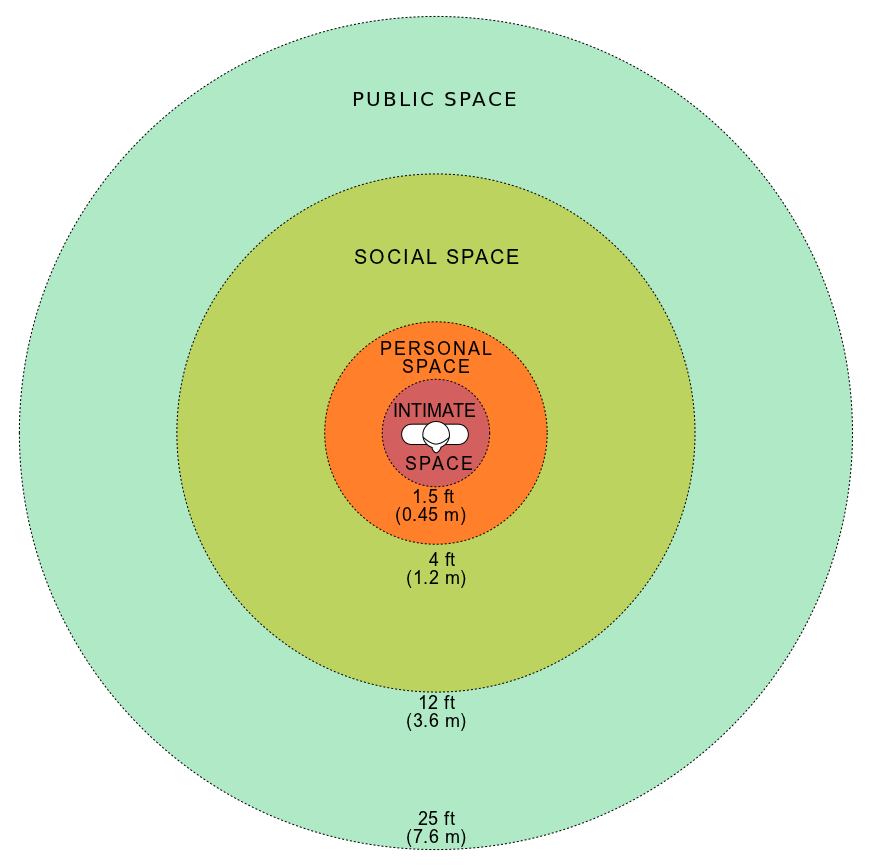
\includegraphics[scale=0.4]{../images/Personal_Space.png}
\caption{Edward T Hall's `reaction bubbles'}
\label{fig:personalSpace}
\end{figure}


\subsection{Classes of Evacuation Behaviour}
\label{Res:subsec:behaviourClasses}
The MASSEgress framework \cite{MultiAgentFramework,PanMASSEgressThesis,IndivBehaviourPseudo} defines three classes of evacuation behaviour which will be considered in this projects behavioural model for agents. These are \emph{competitive behaviour}, \emph{queueing} and \emph{herding}.

\subsubsection{Competitive Behaviour}
\label{Res:subsubsec:competitive}
Competitive behaviour is observed when individuals attempt to force their own exit by competing with others. This includes pushing, moving at an unsafe speed towards exits, etc. Such behaviour generally reduces the efficiency of egress, especially at narrow doorways or other tight spaces\cite{BottleneckStudy}, compared to exiting in a non-competitive (queuing) manner \cite{EgressBehaviourKirchner}.\\
In general this behaviour emerges when a person is highly stressed and perceives an urgent need to evacuate. However an individual can also take up competitive behaviour as a result of social proof, if other individuals around them are acting competitively.
\subsubsection{Queueing}
\label{Res:subsubsec:queueing}
This can be seen as the converse of competitive behaviour. It is characterised by a group organising themselves to facilitate efficient and safe passage through an exit.
\subsubsection{Herding}
\label{Res:subsubsec:herding}
Broadly speaking one can define herding as "the alignment of the thoughts or behaviours of individuals in a group (herd) through local interaction and without centralized coordination" \cite{HerdingInHumans}. Again social proof is a key contributor to the emergence of this behaviour. When an individual has a high degree of uncertainty they will follow the crowd.\\
Unlike other behaviours herding can be either adaptive or non-adaptive depending on the context in which it occurs. Suppose that an individual is following a crowd through an exit. It is possible that this exit is the correct way to proceed, so this choice has aided the person's egress. Equally it may lead to a dead end.

\subsection{Unifying These Concepts In A Behavioural Model}
\label{Res:subsec:unifyingParameters}
We have discussed some of the properties of an individual and groups (such as panic, urgency to exit, etc.) which affect the behaviours exhibited in the evacuation process.\\
For modelling purposes, these factors are unified into a single parameter which shall be referred to as `evacuation stress'. This can be expressed as a percentage where 0 is equivalent to an individual being in regular day-to-day conditions, whereas 100 represents an individual in blind panic acting almost entirely on instinct. Of course these two extremes are unlikely to occur in practice.\\
The reason for this extreme simplification is to limit the possible conditions which must be checked in decision making. The more attributes an agent possesses which may affect decision making there are, the more conditions must be checked at each decision making stage. Even a small number of variables can lead to an very large set of possible outcomes which all must be checked. This can exponentially increase both the complexity of the behavioural model for the programmer and the computational complexity of making a decision.

\subsection{The Perceive, Decide, Act Process}
\label{Res:subsec:perceiveDecideAct}
The decision making process for each agent can be expressed in three stages:
\begin{enumerate}
  \item{\textbf{Perceive}: the agent scans the area around themselves for visible goals or other information. This produces a set of goals in sight.}
  \item{\textbf{Decide}: based on what they can perceive and their current level of evacuation stress, the agent chooses an action with which to proceed.}
  \item{\textbf{Act}: the agent carries out this action.}
\end{enumerate}
An example of this procedure is as follows:
\begin{enumerate}
  \item{An agent scans the room they are in. They perceive two exits, one with only two people moving through it, the other with twenty people waiting at it.}
  \item{The agents current evacuation stress is high enough that they will engage in herding behaviour. They decide to move toward the most crowded of the two doors.}
  \item{The agent plans their route to this destination and initiates the movement.}
\end{enumerate}
 The implementation of this theory is discussed in the Implementation section.

%\bibliographystyle{unsrt}
%\bibliography{references}
%\end{document}
